\documentclass[a4paper,11pt]{article}
\usepackage[utf8]{inputenc}
\usepackage[total={17cm,24cm}, top=3cm, left=2cm]{geometry}
\usepackage[czech]{babel}
\usepackage{times}
\usepackage{hyperref}
\usepackage{multirow}
\usepackage[ruled, czech, linesnumbered, noline, longend]{algorithm2e}
\usepackage{graphicx}
\usepackage{epsfig}
\usepackage{lscape}
\usepackage{pdflscape}


\begin{document}
    \begin{titlepage}
        \begin{center}
            \textsc{\Huge ~Vysoké učení technické v Brně \\[0.3em]
            \huge{Fakulta informačních technologií}}\\
            \vspace{\stretch{0.382}}
            {\LARGE Typografie a publikování\,--\,3. projekt\\[0.3em]
            \Huge{Tabulky a obrázky}}
            \vspace{\stretch{0.618}}
        \end{center}
        {\Large\today \hfill Assatulla Dias }
    \end{titlepage}
    \newpage
    
    \section{Úvodní strana}
    Název práce umístěte do zlatého řezu a nezapomeňte uvést \uv{dnešní} datum a vaše jméno a přímení

    \section{Tabulky}
    Pro sázení tabulek můžeme použít bud' prostředí~\verb|tabbing|~nebo prostředí~\verb|tabular|
    
    \subsection{Prostředí \texttt{tabbing}}
    Při použití~\verb|tabbing|~vypadá tabulka následovně:
    \begin{tabbing}
        \label{tabbing:Ovoce}
        \textbf{Ovoce}\=\qquad\qquad\quad\textbf{Cena}\=\qquad\textbf{Množství} \\
        Jablka\>\qquad\qquad\quad25,90\>\qquad3 kg \\
        Hrušky\>\qquad\qquad\quad27,40\>\qquad2,5 kg \\
        Vodní melouny\>\qquad\qquad\quad35,--\>\qquad1 kus \\
    \end{tabbing}
    Toto prostředí se dá také použít pro sázení algoritmů, ovšem vhodnější je použít prostředí \verb|algorithm| nebo \verb|algorithm2e| (viz sekce 3)
    
    \subsection{Prostředí \texttt{tabular}} 
    Další možností, jak vytvořit tabulku, je použít prostředí \verb|tabular|. Tabulky pak budou vypadat takto\footnote{Kdyby byl problem s \texttt{cline} , zkuste se podívat třeba sem: \href{http://www.abclinuxu.cz/tex/poradna/show/325037}{http://www.abclinuxu.cz/tex/poradna/show/325037}.}:
    \newline
     \begin{table}[h]
        \centering
        \catcode`\-=12
        
        \begin{tabular}[]{| c | c | c |} 
        \hline
                & \multicolumn{2}{| c |}{\textbf{Cena}} \\
            \cline{2-3}
        \textbf{Měna} & \textbf{nákup} & \textbf{prodej} \\
        \hline
        EUR & 24,775 & 25,943 \\
        GBP & 29,394 & 30,492 \\
        USD & 22,423 & 23,661 \\
        \hline
        \end{tabular}
        \caption{Tabulka kurzů k dnešnímu dni}
        \label{table:Kurz}
     \end{table}
     
     \begin{table}[h]
         \catcode`\-=12
         \begin{tabular}{| c | c |}
                \hline
                $A$ & $\neg A$ \\
                \hline
                \textbf{P} & N \\
                \hline
                \textbf{O} & O \\
                \hline
                \textbf{X} & X \\
                \hline
                \textbf{N} & P \\
                \hline
         \end{tabular}
        \catcode`\-=12
         \begin{tabular}{| c | c | c | c | c | c |}
                \hline
                \multicolumn{2}{| c |}{\multirow{2}{*}{$A \land B$}} & \multicolumn{4}{| c |}{$B$} \\
                \cline{3-6}
                \multicolumn{2}{| c |}{} & \textbf{P} & \textbf{O} & \textbf{X}	& \textbf{N} \\ \hline
                \multirow{4}{*}{$A$} & \textbf{P} & P & O & X & N \\
                \cline{2-6}
                                     &\textbf{O}  & O & O & N & N \\
                \cline{2-6}
                                     &\textbf{X}  & X & N & X & N \\
                \cline{2-6}
                                     &\textbf{N}  & N & N & N & N \\
                \hline
         \end{tabular}
        \catcode`\-=12
         \begin{tabular}{| c | c | c | c | c | c |}
                \hline
                \multicolumn{2}{| c |}{\multirow{2}{*}{$A \lor B$}} & \multicolumn{4}{| c |}{$B$} \\
                \cline{3-6}
                \multicolumn{2}{| c |}{} & \textbf{P} & \textbf{O} & \textbf{X}	& \textbf{N} \\ \hline
                \multirow{4}{*}{$A$} & \textbf{P} & P & P & P & P \\
                \cline{2-6}
                                     &\textbf{O}  & P & O & P & O \\
                \cline{2-6}
                                     &\textbf{X}  & P & P & X & X \\
                \cline{2-6}
                                     &\textbf{N}  & P & O & X & N \\
                \hline
         \end{tabular}
         \catcode`\-=12
         \begin{tabular}{| c | c | c | c | c | c |}
                \hline
                \multicolumn{2}{| c |}{\multirow{2}{*}{$A \rightarrow B$}} & \multicolumn{4}{| c |}{$B$} \\
                \cline{3-6}
                \multicolumn{2}{| c |}{} & \textbf{P} & \textbf{O} & \textbf{X}	& \textbf{N} \\ \hline
                \multirow{4}{*}{$A$} & \textbf{P} & P & O & X & N \\
                \cline{2-6}
                                     &\textbf{O}  & P & O & P & O \\
                \cline{2-6}
                                     &\textbf{X}  & P & P & X & X \\
                \cline{2-6}
                                     &\textbf{N}  & P & P & P & P \\
                \hline
         \end{tabular}
         \caption{Protože Kleeneho trojhodnotová logika už je \uv{zastralá}, uvádíme si zde příklad čtyřhodnotové logiky }
         \label{table:logic}
     \end{table}
     \pagebreak
     \newpage
     
     
     \section{Algoritmy}
     Pokud budeme chtít vysázet algoritmus, můžeme použít prostředí \verb|algorithm|\footnote{
        Pro nápovědu, jak zacházet s prostředím \texttt{algorithm}, můžeme zkusit tuhle stránku:\\ \href{http://ftp.cstug.cz/pub/tex/CTAN/macros/latex/contrib/algorithms/algorithms.pdf}{http://ftp.cstug.cz/pub/tex/CTAN/macros/latex/contrib/algorithms/algorithms.pdf}.
    } nebo \verb|algorithm2e|\footnote{
        Pro \texttt{algorithm2e} zase tuhle: \href{http://ftp.cstug.cz/pub/tex/CTAN/macros/latex/contrib/algorithm2e/doc/algorithm2e.pdf}{http://ftp.cstug.cz/pub/tex/CTAN/macros/latex/contrib/algorithm2e/doc/algorithm2e.pdf}.
    }. \\
     Příklad použití prostředí \verb|algorithm2e| viz Alhoritmus 1. \\
    
    \begin{algorithm}
        \label{algorithm:FastSLAM}
     \caption{\textsc{FastSLAM}}
     \KwIn{$(X_{t-1},u_t,z_t)$}
     \KwOut{$X_t$}
     
    \SetNlSkip{-1.0em}
    \SetNlSty{}{}{:}
    \Indp\Indp
    \BlankLine
     $ \overline{X_t} = X_t = 0 $ \\
     \For{$k = 1$ \textup{to} $M$} {
            $x^{[k]}_{t} = $ \textit{sample\_motion\_model}$(u_t,x^{[k]}_{t-1})$ \\
            $\omega^{[k]}_{t} = $ \textit{measurement\_model}$(z_t,x^{[k]}_{t},m_{t-1})$ \\
            $m^{[k]}_{t} = updated\_occupancy\_grid(z_t,x^{[k]}_{t},m_{t-1}^{[k]})$ \\
            $\overline{X_t} = \overline{X_t} + \langle x_{x}^{[m]}, \omega_{t}^{[m]}\rangle$
            }
    \For{$k = 1$ \textup{to} $M$}{
            draw $i$ with probability $\approx \omega_{t}^{[i]}$ \\
            add $\langle x_{x}^{[k]}, m_{t}^{[k]}\rangle$ to $X_t$ \\
    }
    \Return{$X_t$}
    \end{algorithm}
    
    
    \section{Obrázky}
    Do našich článků můžeme samozřejmě vkládat obrázky. Pokud je obrázkem fotografie, můžeme klidně použít bitmapový soubor. Pokud by to ale mělo být nějaké schéma nebo něco podobného, je dobrým zvykem takovýto obrázek vytvořit vektorově.
    
    \begin{figure}[h]
        \centering
        \scalebox{0.4}{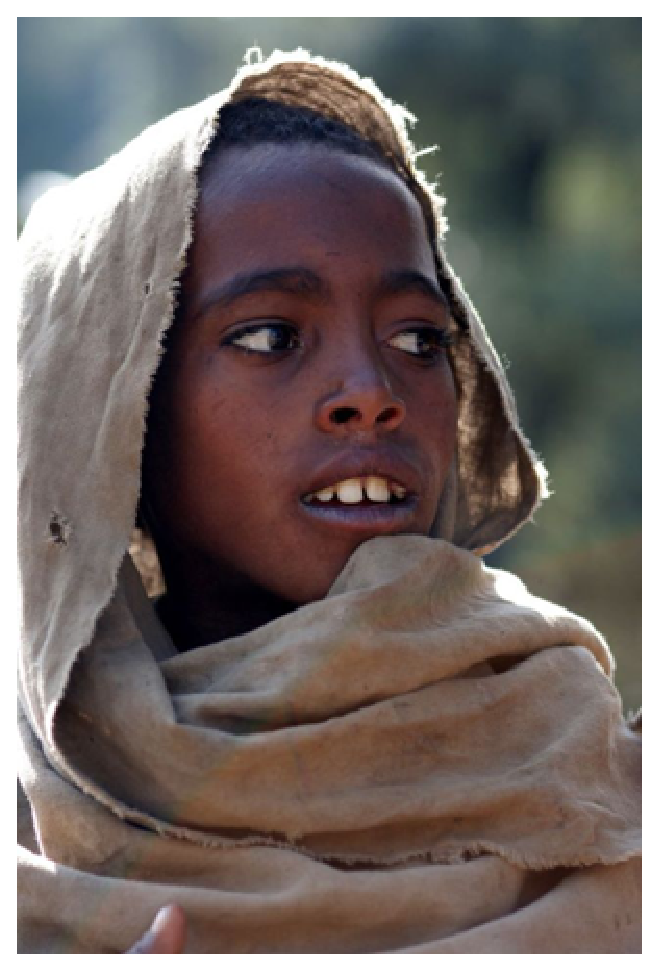
\includegraphics{img/etiopan.eps}
            \reflectbox{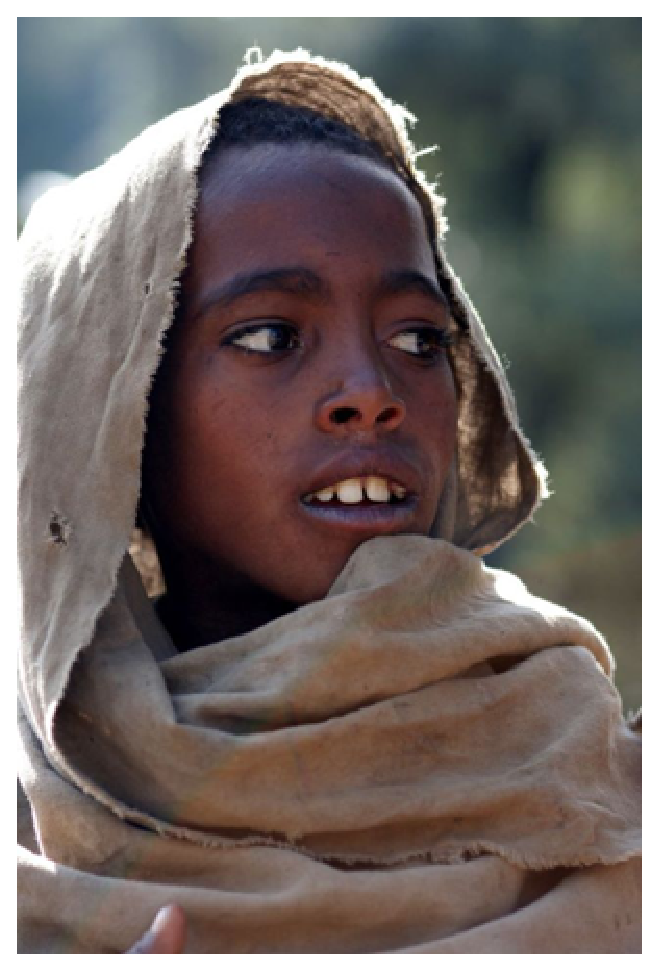
\includegraphics{img/etiopan.eps}}
        }
        \caption{Malý Etiopánek a jeho bratříček}
        \label{fig:Etiopanek}
    \end{figure}
    \newpage
     \bigskip Rozdíl mezi vektorovým \dots \\
    \begin{figure}[h]
        \centering
        \scalebox{0.4}{
\includegraphics{img/oniisan.eps}}
        \caption{Vektorový obrázek}
        \label{fig:vek-obrazek}
    \end{figure} \\
    \dots a bitmapovým obrázkem \\
    \begin{figure}[h]
        \centering
        \scalebox{0.6}{
\includegraphics{img/oniisan2.eps}}
        \caption{Bitmapový obrázek}
        \label{fig:bit-obrazek}
    \end{figure}\\
    se projeví například při zvětšení. 
    
    Odkazy (nejen ty) na obrázky \ref{fig:Etiopanek},\ref{fig:vek-obrazek} a \ref{fig:bit-obrazek}, na tabulky \ref{table:Kurz} a \ref{table:logic} a také na algoritmus \ref{algorithm:FastSLAM} jsou udělány pomocí křížových odkazů. Pak je ovšem potřeba zdrojový soubor přeložit dvakrát.
    
    Vektotové obrázky lze vytvořit i přímo v \LaTeX u, například pomocí prostředí \verb|picture|.
    


    \begin{landscape}
        \begin{figure}[h]
            \setlength{\unitlength}{1mm}
            \centering
            \begin{picture}(200,100)
                \linethickness{1pt}
                \put(0,0){\framebox(200,100)}
                \linethickness{1.5mm}
				\put(4,14){\line(1,0){192}}
				
				\linethickness{0.4mm}
				%dum
				\put(24, 14){\line(0, 0){36}}
				\put(24, 50){\line(1, 0){70}}
				\put(94,14){\line(0,0){36}}
				\put(30,14){\line(0,0){15}}
				\put(30,29){\line(1,0){8}}
				\put(38,14){\line(0,0){15}}
				\put(36,22){\circle*{1}}
				%okno
				\put(40,40){\circle{9}}
				\put(40,40){\circle{10}}
				\put(36,40){\line(1,0){8}}
				\put(40,36){\line(0,0){8}}
				%garage
				\multiput(54, 40)(0, -6){5}{\line(1, 0){40}}
				\put(54,14){\line(0,0){26}}
				%strecha
				\put(24, 50){\line(1, 1){35}}
				\put(94, 50){\line(-1, 1){35}}
				\put(26, 50){\line(1, 1){33}}
				\put(92, 50){\line(-1, 1){33}}
			    \put(84,60){\line(0,1){20}}
			    \put(74,70){\line(0,1){10}}
			    \put(74,80){\line(1,0){10}}
				
				
				%slunce
				\linethickness{0.1mm}
				\put(180,80){\circle{20}}
				\put(168,68){\line(1,1){6}}
				\put(168,92){\line(1,-1){6}}
				\put(186,74){\line(1,-1){6}}
				\put(186,86){\line(1,1){6}}
				\put(188,80){\line(1,0){7}}
				\put(172,80){\line(-1,0){7}}
				\put(180,88){\line(0,1){7}}
				\put(180,72){\line(0,-1){7}}
            \end{picture}
            \caption{Vektorový obrázek moderího bydlení vhodného pro 21. století. (Bud’to vytvoŕte stejný obrázek, anebo nakreslete pomocí \texttt{picture} váš vlastní domov.) \\
            Komentář: Všechna krása je v jednoduchosti a harmonii :)}
            \label{fig:myhome}
        \end{figure}
    \end{landscape}
    
\end{document}
